%!TeX options = -shell-escape
\documentclass{article}
\usepackage{tikz}
\usetikzlibrary{external}
\tikzexternalize
\begin{document}
\begin{center}
	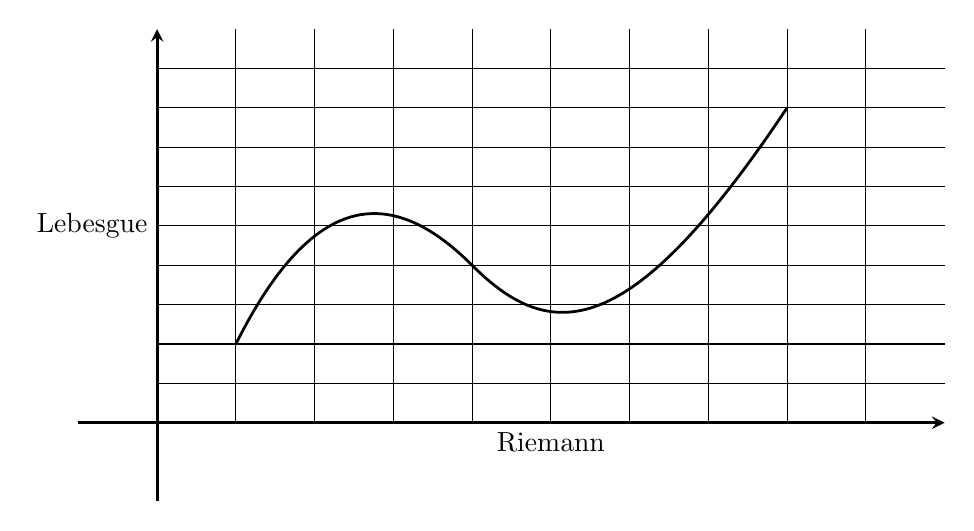
\begin{tikzpicture}
		\draw [-{stealth[black]}, line width=1pt] (-1, 0) -- (10, 0);
		\draw [-{stealth[black]}, line width=1pt] (0, -1) -- (0, 5);
		\draw [line width=1pt] (1, 1) .. controls (2, 3) and (3, 3) .. (4, 2) 
									  .. controls (5, 1) and (6, 1) .. (8, 4);
		\foreach \x in {1,...,9}
			\draw (0, \x/2) -- (10, \x/2);

		\foreach \y in {1,...,9}
			\draw (\y, 0) -- (\y, 5);

		\node[align=justify, below] at (5, 0) {Riemann};
		\node[align=justify, left] at (0, 2.5) {Lebesgue};
	\end{tikzpicture}
\end{center}
\end{document}

